% -*- Mode:TeX -*-

%% IMPORTANT: The official thesis specifications are available at:
%%            http://libraries.mit.edu/archives/thesis-specs/
%%
%%            Please verify your thesis' formatting and copyright
%%            assignment before submission.  If you notice any
%%            discrepancies between these templates and the 
%%            MIT Libraries' specs, please let us know
%%            by e-mailing thesis@mit.edu

%% The documentclass options along with the pagestyle can be used to generate
%% a technical report, a draft copy, or a regular thesis.  You may need to
%% re-specify the pagestyle after you \include  cover.tex.  For more
%% information, see the first few lines of mitthesis.cls. 

%\documentclass[12pt,vi,twoside]{mitthesis}
%%
%%  If you want your thesis copyright to you instead of MIT, use the
%%  ``vi'' option, as above.
%%
%\documentclass[12pt,twoside,leftblank]{mitthesis}
%%
%% If you want blank pages before new chapters to be labelled ``This
%% Page Intentionally Left Blank'', use the ``leftblank'' option, as
%% above. 

%\documentclass[12pt,twoside]{report}
%\documentclass[a4paper, 11pt]{scrartcl}
\documentclass[a4paper, 11pt, bibliography=totoc, twoside]{scrreprt}
\usepackage[top=1cm,bottom=1cm,includeheadfoot,includefoot]{geometry}
%\documentclass{report}
\usepackage{lgrind}
\usepackage{amsmath}
\usepackage{amssymb}
\usepackage{mathtools}
\usepackage{bm}
\usepackage{esvect}
\usepackage{graphicx}
\usepackage{wrapfig}
\usepackage{caption}
\usepackage{subcaption}
\usepackage{float}
\usepackage{listings}
\usepackage{rotating}
\usepackage[german]{babel}
\usepackage{geometry}
\usepackage{url}
\usepackage{hyperref}
\usepackage{xcolor}
\usepackage{tikz}

\graphicspath{ {../pics/} }
%% These have been added at the request of the MIT Libraries, because
%% some PDF conversions mess up the ligatures.  -LB, 1/22/2014
\usepackage{cmap}
%%\usepackage[T1]{fontenc}
\pagestyle{plain}

%% This bit allows you to either specify only the files which you wish to
%% process, or `all' to process all files which you \include.
%% Krishna Sethuraman (1990).

\newcommand*\circled[1]{\tikz[baseline=(char.base)]{
		\node[shape=circle,draw,inner sep=2pt] (char) {#1};}}
	
%\DeclareCaptionType{mycapequ}[][List of equations]
%\captionsetup[mycapequ]{labelformat=empty}


% Define colors for syntax highlighting
\definecolor{codegreen}{rgb}{0,0.6,0}
\definecolor{codegray}{rgb}{0.5,0.5,0.5}
\definecolor{codepurple}{rgb}{0.58,0,0.82}
\definecolor{backcolour}{rgb}{0.95,0.95,0.92}

% Settings for C++ code
\lstset{
	language=C++,
	basicstyle=\small\ttfamily,
	keywordstyle=\color{blue},
	stringstyle=\color{codepurple},
	commentstyle=\color{codegreen},
	backgroundcolor=\color{backcolour},
	numbers=left,
	numberstyle=\tiny\color{codegray},
	stepnumber=1,
	breaklines=true,
	breakatwhitespace=false,
	tabsize=2,
	showstringspaces=false,
	captionpos=b,
    columns=fullflexible % Allows the width to exceed the page width
}



\begin{document}
%Erklärungsseite

%left Blank Page
\newcommand{\leftblankpage}
{
	\begingroup
	\clearpage
	\vspace*{60mm}
	\noindent
	\centering
	\makebox[0.5\textwidth][c]{\emph{This page intentionally left blank}}
	\clearpage
	\endgroup
}

%\subtitle{\LARGE Entwicklung eines Virtual Reality Videospiels für das HTC Vive VR System}
\subtitle{\LARGE Digitale Bildverarbeitung WS2023/24}
\title{Morphing mit Beier-Neely}
\author{Michael Eggers, Johann Rittenschober, Kevin}
\date{\today}

\maketitle

%\leftblankpage



\begingroup
\begin{figure}[h]
	\centering
		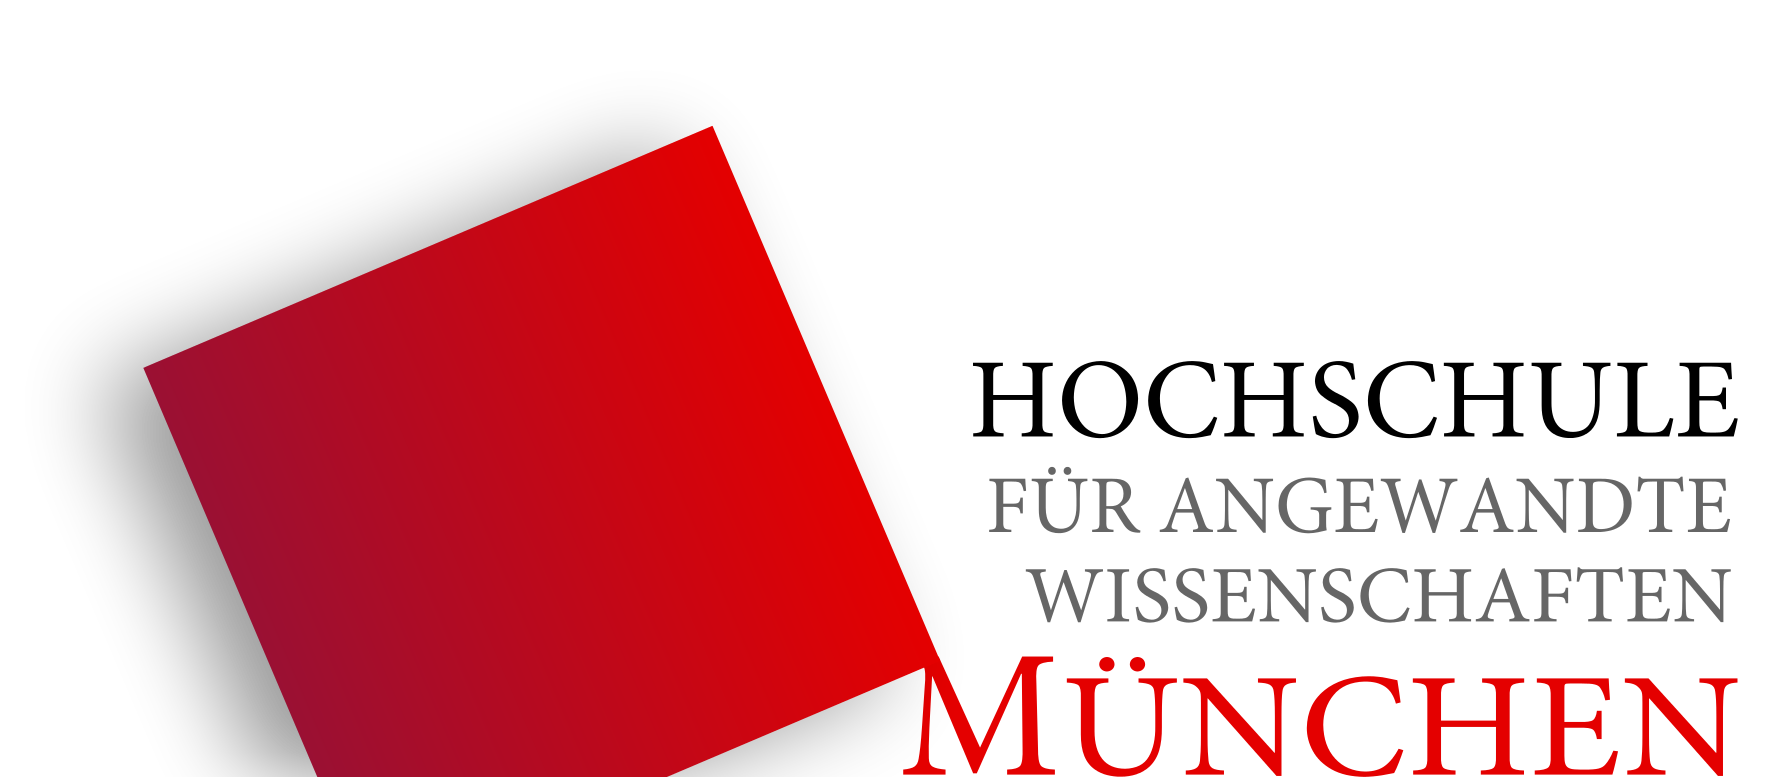
\includegraphics[width=1.0\textwidth]{Hochschule_Muenchen_Logo}
	\label{fig:HM_FK04_Logo}
\end{figure}
\let\clearpage\relax
\chapter*{Erklärung}
\noindent
Hiermit erklären wir, dass die vorliegenden Arbeit selbstständig verfasst, noch nicht anderweitig für Prüfungszwecke vorgelegt, keine anderen als die angegebenen Quellen oder Hilfsmittel benutzt sowie wörtliche und sinngemäße Zitate als solche gekennzeichnet wurden.
\par
\vspace{20mm}
\noindent
\makebox[0.0\textwidth][l]{Michael Eggers, Johann Rittenschober, Kevin}
%\makebox[0.99\textwidth][r]{Oberbrunn, 28.02.2017}
\makebox[0.99\textwidth][r]{München, \today}

\vspace{20mm}

\noindent
\makebox[0.0\textwidth][l]{Matrikelnummer: 00322614}
\par
\noindent
\makebox[0.0\textwidth][l]{Studiengruppe: Master Informatik VZ/TZ}
\endgroup


\section*{Zusammenfassung}

schreiben \cite{beierneely} test

\section*{Abstract}

write

\pagestyle{plain}
  % -*- Mode:TeX -*-
%% This file simply contains the commands that actually generate the table of
%% contents and lists of figures and tables.  You can omit any or all of
%% these files by simply taking out the appropriate command.  For more
%% information on these files, see appendix C.3.3 of the LaTeX manual. 
\tableofcontents
\newpage
\listoffigures
\newpage
\listoftables




\chapter{Festlegung der Features}

Wie eingangs beschrieben handelt es sich um einen Feature basierten Algorithmus. Das hei\ss t, dass die
Merkmale eines Objekt im Bild, welches transformiert werden soll, zunächst erfasst werden müssen.
Beier und Neely nutzen dazu eine Liste aus gerichteten Linienpaaren: Einer Linie im Quellbild wird genau eine
Linie im Zielbild zugeordnet. Dabei werden die Linienpaare so platziert, sodass sie ein Merkmal
in den Bildern beschreiben. Zum Beispiel werden die Haaransätze der beiden Personen in Quell- und Zielbild
als Merkmale deklariert: Das Linienpaar wird dementsprechend gesetzt, siehe \ref{fig:linepairs}.

\begin{figure}[htbp]
	\centering
	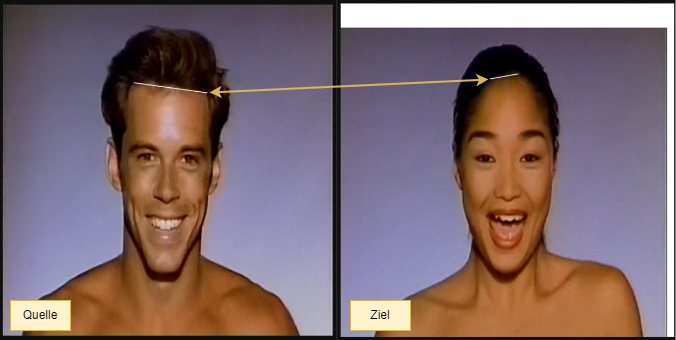
\includegraphics[width=0.9\textwidth]{linienpaare.drawio.png}
	\caption{Setzen eines Linienpaares}
	\label{fig:linepairs}
\end{figure}
Es ist wichtig zu beachten, dass die Linienpaare gerichtet sind. Die Linien besitzen also sowohl
Anfangs- als auch Endpunkt. Abbildung \ref{fig:linepairsfinal} zeigt die Linienpaare, welche für dass Resultat in
\ref{fig:morph} verantwortlich waren.
\begin{figure}[htbp]
	\centering
	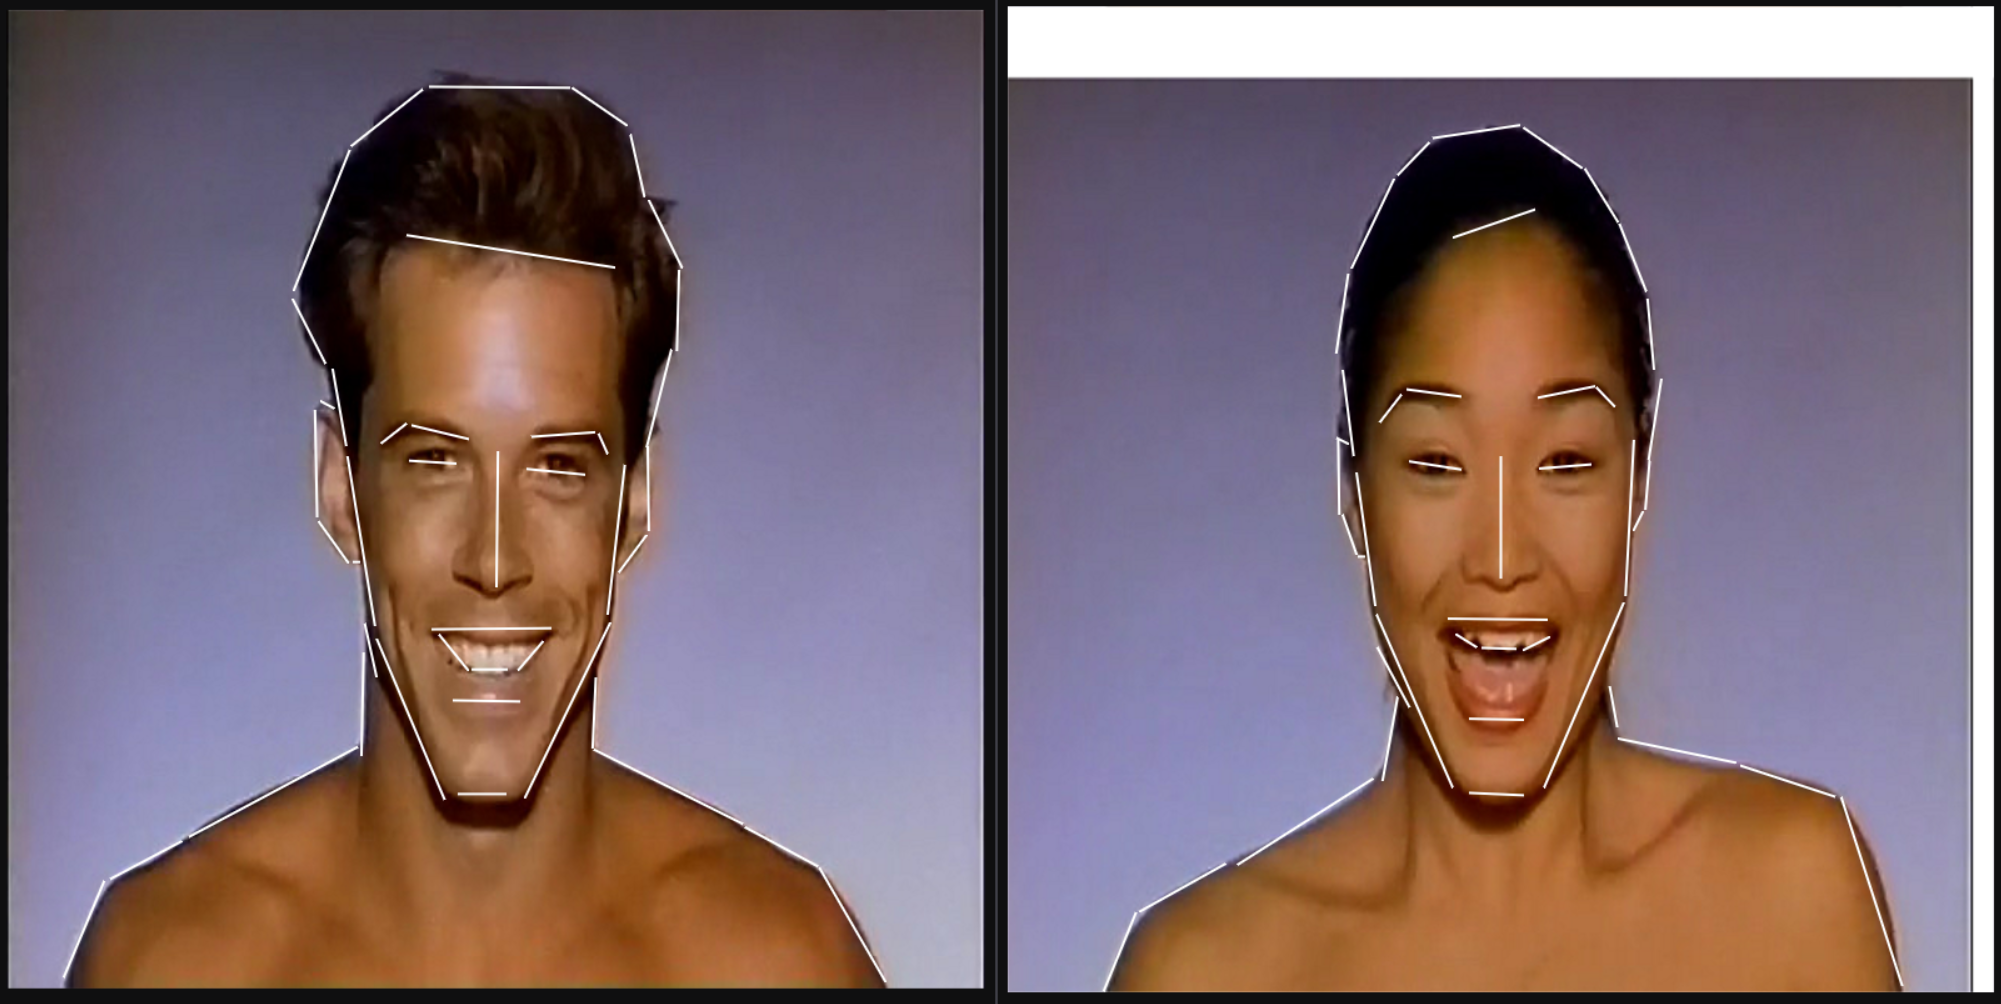
\includegraphics[width=0.9\textwidth]{linienpaarefinal.png}
	\caption{Finale Menge an Linienpaaren}
	\label{fig:linepairsfinal}
\end{figure}




\chapter{Warping der Bilder}

Sobald die Linienpaare gesetzt wurden, kann der eigentliche Algorithmus gestartet werden. Die Pixel
des Quellbildes werden in Richtung der Linienpositionen des Zielbildes verschoben. Und die Pixel
des Zielbildes wiederum werden in Richtung der Linienpositionen des Quellbildes verschoben.
Dies ist ein iterativer Prozess. Je mehr Iterationen gewählt werden, desto flie \ss ender ist
die Verzerrung.
Fuer jeden Pixel im Bild wird jede Linie in Betracht gezogen. Alle Linien haben also einen gewissen Einfluss auf
das Warping eines Pixels. Die Laufzeitkomplexitaet
des Beier-Neely Algorithmus errechnet sich aus
$\mathcal{O}(numPixels \cdot numLines)$.
Der Einfluss einer Linie auf einen Pixel kann mit einem
von Beier-Neely entwickelten Gewicht festgelegt werden
\cite{beierneely}:

\begin{equation}
	weight = \left(\frac{length^{p}}{a+dist}\right)^{b}
\end{equation}

a, b, p sind Konstanten, die einmalig gesetzt werden.

\begin{itemize}
	\item \textbf{length}: Laenge der Linie
	\item \textbf{dist}: senkrechter Abstand des Pixels zur Linie
	\item \textbf{a}: Bestimmt den Einfluss der senkrechten Distanz
	auf das Gewicht. Wenn a nahe 0 ist, so werden Pixel, die auf der
	Linie liegen mit einem Gewicht von nahezu $\infty$ beeinflusst.
	\item \textbf{b}: Kontrolliert den Fall-Off der Linien. Ist b
	nahe 0, tragen alle Linien, gleich Ihrer senkrechten Distanz zum
	Pixel, gleichmaessig zur Verzerrung des jenes Pixels bei.
	Grosse Werte (es wird nicht erwaehnt, was gross ist), fuehren
	zu einem hoeheren Gewicht, je naeher der Pixel sich an
	der jeweiligen Linie befindet.
	\item \textbf{p}: Regelt, ob sich die Linienlaenge auf das Gewicht
	auswirkt. Bei einem Wert von 0 wird $length^{p}$ offensichtlich 1
	und das Gewicht ist unabhaengig zur Linienlaenge.
\end{itemize}

Wie die Parameter festgelegt werden kommt auf die in den Bildern
vorhandenen Features an und erfordert in der Regel ein wenig
ausprobieren. Beispielsweise haben sich die Werte 
a = 0, b = 3.1 und p = 0 fuer das Bilderset aus Abbildung
\ref{fig:linepairsfinal} in unseren Tests bewaehrt.
Die Linien koennen linear interpoliert werden, wie Abbildung \ref{fig:linearinterpolation}zeigt. 
\begin{figure}[htb]
	\centering
	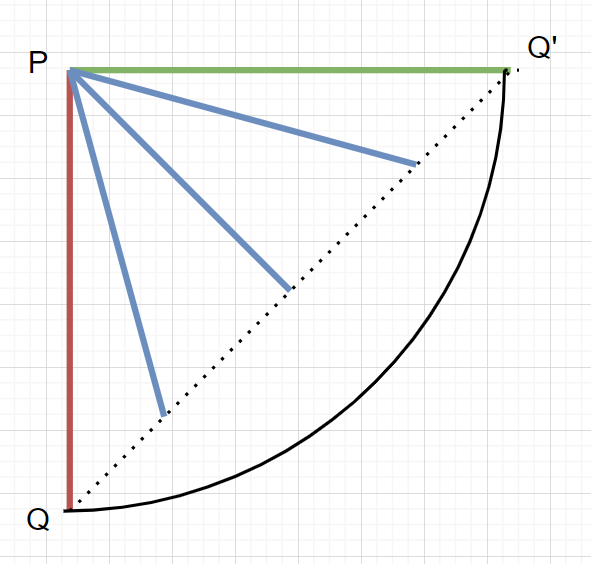
\includegraphics[width=0.5\textwidth]{linearinterpolation.drawio.png}
	\caption{Lineare Interpolation zwischen Ziellinie $\overline{PQ}$ und Quelllinie $\overline{PQ'}$}
	\label{fig:linearinterpolation}
\end{figure}
Durch diese Art der Interpolation entsteht jedoch bei
Rotationen ein Fehler, wie man in \ref{fig:linearinterpolation} sehen kann: Die linear
interpolierten Linien nehmen faelschlicherweise
an Laenge ab. In unseren praktischen Tests hat sich
dieses Problem als nicht gravierend herausgestellt.
Fuer unsere Implementierung nutzen wir den von Beier und Neely
mitgelieferten Pseudocode. Unsere Implementierung:

\clearpage

\begin{minipage}{\textwidth}
\begin{lstlisting}[language=C++, caption=Beier-Neely in C++, label=bncode, xleftmargin=0.5cm]
for (uint32_t y = 0; y < destImage.m_Height; y++) {
	for (uint32_t x = 0; x < destImage.m_Width; x++) {
		glm::vec2 X = glm::vec2(x, y);
		glm::vec2 DSUM = glm::vec2(0.0, 0.0);
		float weightsum = 0;     
		for (uint32_t i = 0; i < destLines.size(); i++) {
			
			Line& destLine = destLines[i];
			Line& srcLine = sourceLines[i];
			Line interpolatedLine = InterpolateLinesLinear(destLine, srcLine, pct);
			
			glm::vec2 P = destLine.a.pos;
			glm::vec2 Q = destLine.b.pos;
			glm::vec2 srcP = interpolatedLine.a.pos;
			glm::vec2 srcQ = interpolatedLine.b.pos;
			glm::vec2 PX = X - P;
			glm::vec2 PQ = Q - P;
			float PQlength = glm::length(PQ);
			float u = glm::dot(PX, PQ) / (PQlength * PQlength);
			float v = glm::dot(PX, Perpendicular(PQ)) / PQlength;
			glm::vec2 srcPQ = srcQ - srcP;
			glm::vec2 srcX = srcP + u * srcPQ + (v * Perpendicular(srcPQ) / glm::length(srcPQ));
			glm::vec2 D = srcX - X;
			float dist = Distance(u, v, P, Q, X);
			float weight = glm::pow(glm::pow(PQlength, p) / (a + dist), b);
			DSUM += D * weight;
			weightsum += weight;        
		}                
		glm::vec2 srcX = X + DSUM / weightsum;
		if ((uint32_t)srcX.x > destImage.m_Width - 1) srcX.x = float(destImage.m_Width - 1);
		if ((uint32_t)srcX.y > destImage.m_Height - 1) srcX.y = float(destImage.m_Height - 1);
		if ((uint32_t)srcX.x < 0) srcX.x = 0.0f;
		if ((uint32_t)srcX.y < 0) srcX.y = 0.0f;                
		
		glm::ivec3 sourcePixel = sourceImage((uint32_t)srcX.x, (uint32_t)srcX.y);                
		
		unsigned char* newPixel = image.m_Data + (image.m_Channels * (y * image.m_Width + x));
		newPixel[0] = sourcePixel.r;
		newPixel[1] = sourcePixel.g;
		newPixel[2] = sourcePixel.b;
		
	} // ! pixel row
} // ! pixel col    
\end{lstlisting}
\end{minipage}




\chapter{Komposition}

Sind die beiden Bilder erst einmal fertig verzerrt worden, so werden
sie nun, wie eingangs beschrieben, durch eine Kreuzblende 
zusammengefuegt. Zu beachten ist, dass das Zielbild
in Richtung des Quellbildes gewarpt wurde. Die Bildsequenzen
fuer die beiden Bilder sehen dementsprechend folgendermassen
aus:

\begin{figure}[htbp]
	\centering


	
	\begin{subfigure}[b]{0.19\textwidth}
		\centering
		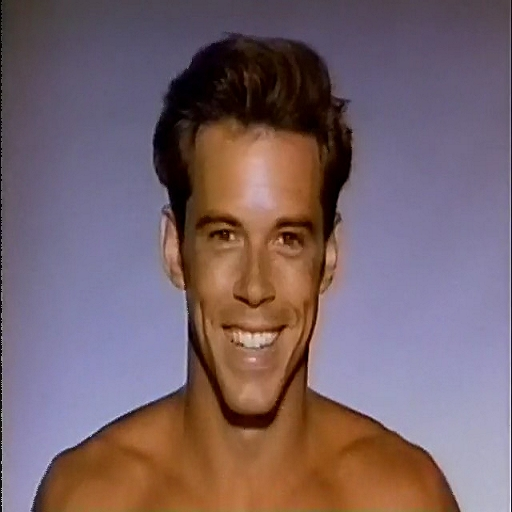
\includegraphics[width=\textwidth]{source/src0.jpg} % Replace 'image1' with your image file name
		\caption{}
	\end{subfigure}
		\begin{subfigure}[b]{0.19\textwidth}
		\centering
		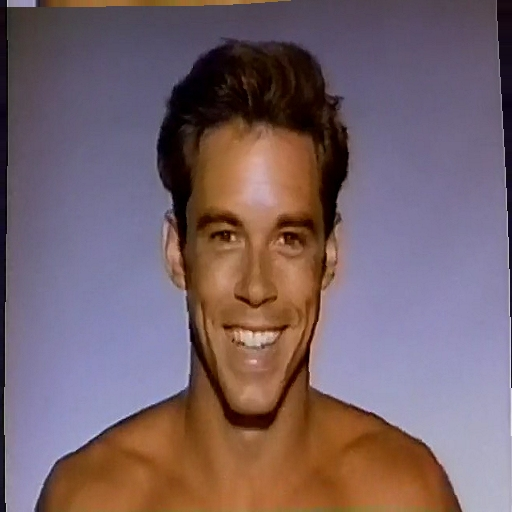
\includegraphics[width=\textwidth]{source/src1.jpg} % Replace 'image1' with your image file name
		\caption{}
	\end{subfigure}
		\begin{subfigure}[b]{0.19\textwidth}
		\centering
		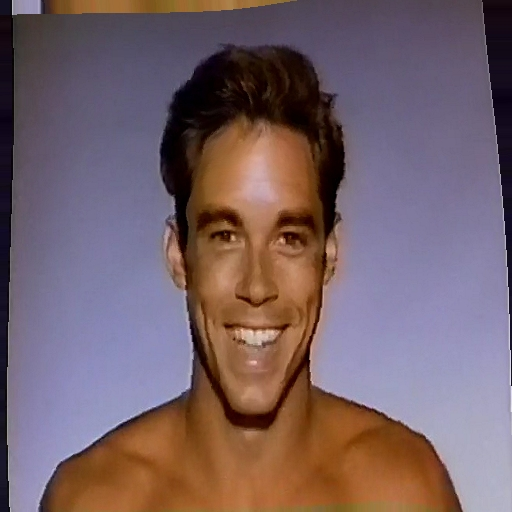
\includegraphics[width=\textwidth]{source/src2.jpg} % Replace 'image1' with your image file name
		\caption{}
	\end{subfigure}
		\begin{subfigure}[b]{0.19\textwidth}
		\centering
		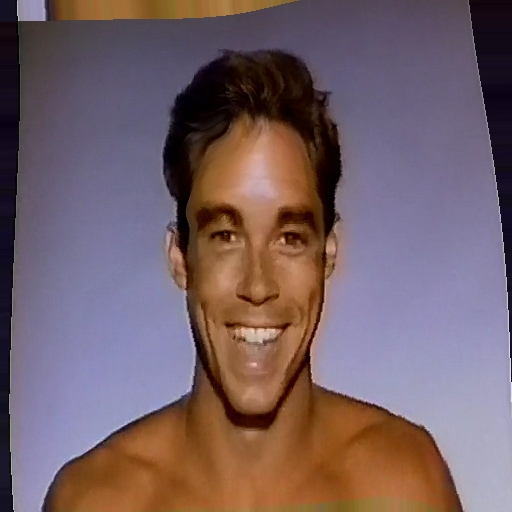
\includegraphics[width=\textwidth]{source/src3.jpg} % Replace 'image1' with your image file name
		\caption{}
	\end{subfigure}
		\begin{subfigure}[b]{0.19\textwidth}
		\centering
		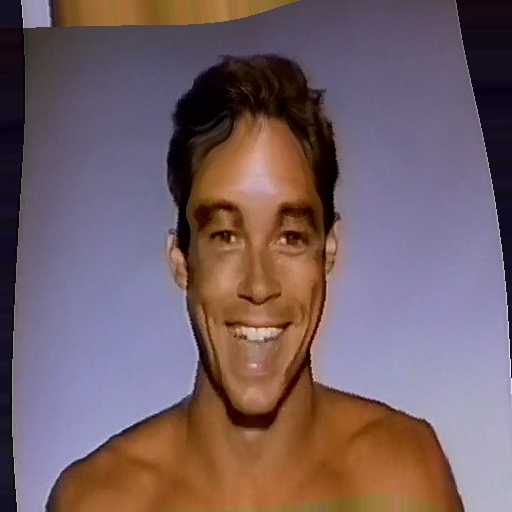
\includegraphics[width=\textwidth]{source/src4.jpg} % Replace 'image1' with your image file name
		\caption{}
	\end{subfigure}
		\begin{subfigure}[b]{0.19\textwidth}
		\centering
		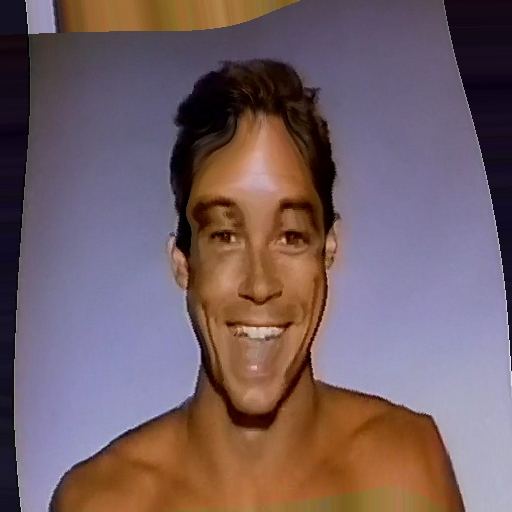
\includegraphics[width=\textwidth]{source/src5.jpg} % Replace 'image1' with your image file name
		\caption{}
	\end{subfigure}
			\begin{subfigure}[b]{0.19\textwidth}
		\centering
		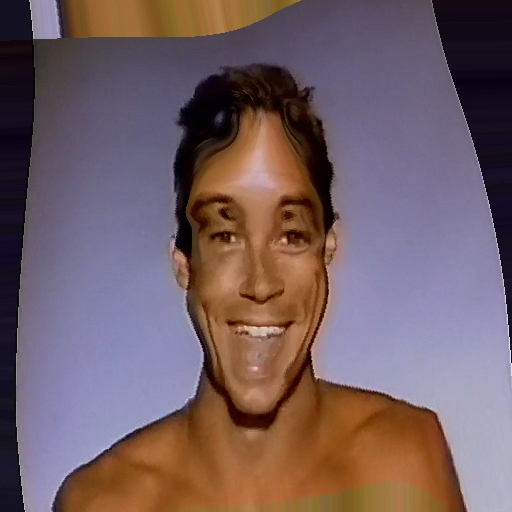
\includegraphics[width=\textwidth]{source/src6.jpg} % Replace 'image1' with your image file name
		\caption{}
	\end{subfigure}
	

	
		\caption{Quell- zu Ziel warps}
	\label{fig:sources}
	\end{figure}
	% Repeat the subfigure environment for each image
	% ... (Add more subfigures for the remaining images)
	
	% Example of a second row
\begin{figure}[htbp]
	\centering

	    	
	\begin{subfigure}[b]{0.19\textwidth}
		\centering
		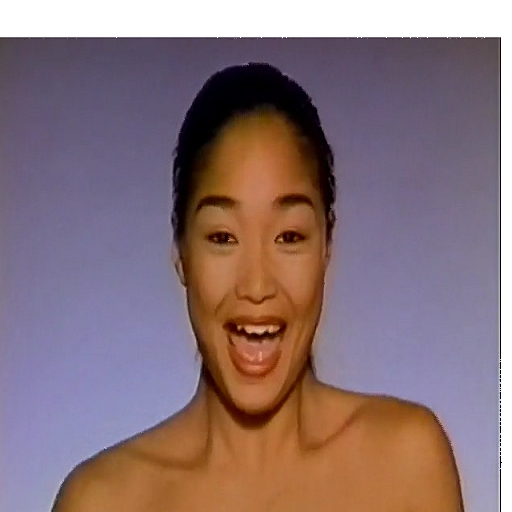
\includegraphics[width=\textwidth]{dst/dest6} % Replace 'image7' with your image file name
		\caption{}
	\end{subfigure}
		\begin{subfigure}[b]{0.19\textwidth}
		\centering
		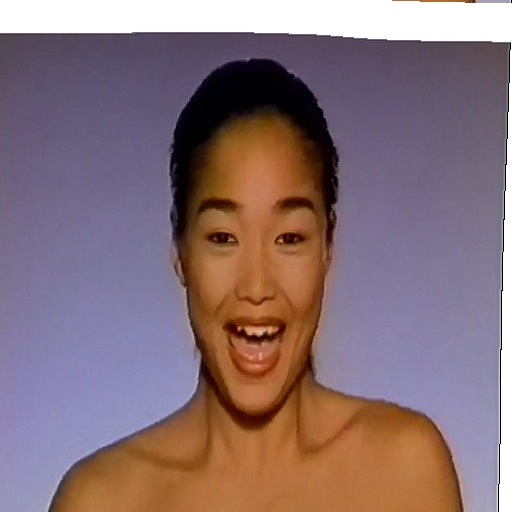
\includegraphics[width=\textwidth]{dst/dest5} % Replace 'image7' with your image file name
		\caption{}
	\end{subfigure}
		\begin{subfigure}[b]{0.19\textwidth}
		\centering
		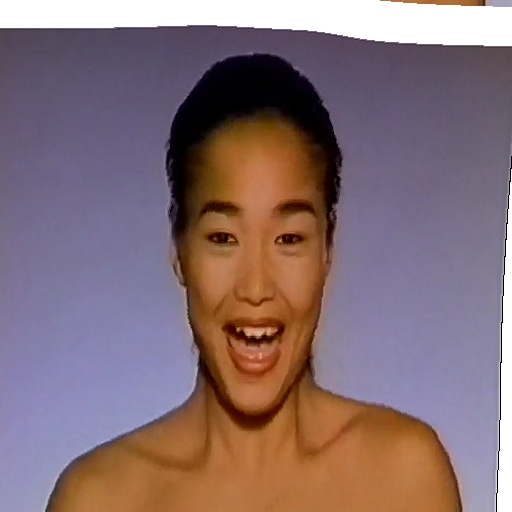
\includegraphics[width=\textwidth]{dst/dest4} % Replace 'image7' with your image file name
		\caption{}
	\end{subfigure}
		\begin{subfigure}[b]{0.19\textwidth}
		\centering
		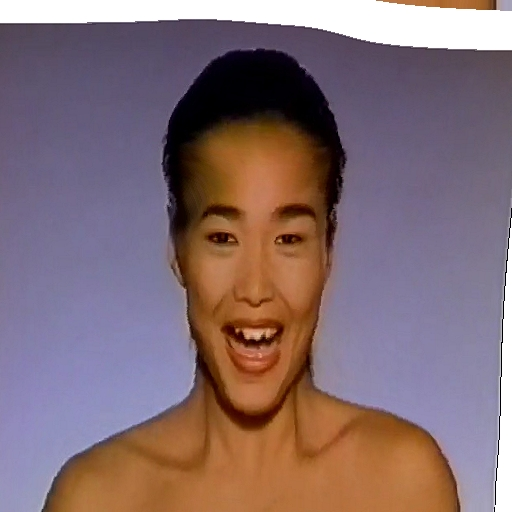
\includegraphics[width=\textwidth]{dst/dest3} % Replace 'image7' with your image file name
		\caption{}
	\end{subfigure}
		\begin{subfigure}[b]{0.19\textwidth}
		\centering
		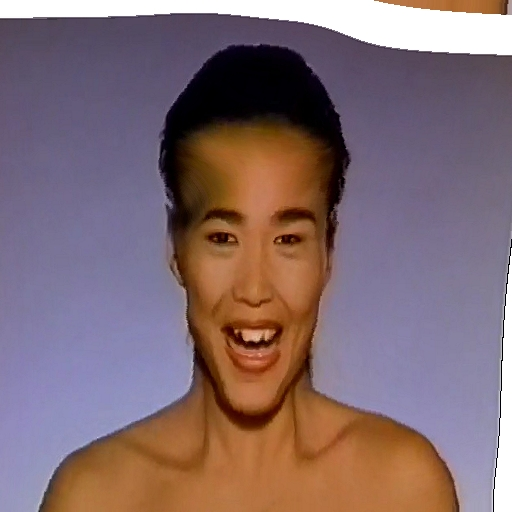
\includegraphics[width=\textwidth]{dst/dest2} % Replace 'image7' with your image file name
		\caption{}
	\end{subfigure}
		\begin{subfigure}[b]{0.19\textwidth}
		\centering
		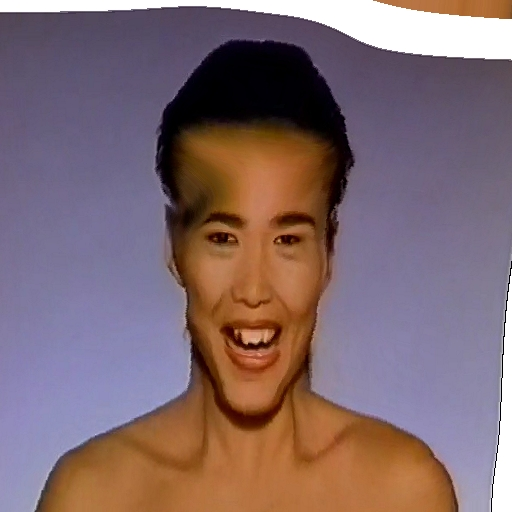
\includegraphics[width=\textwidth]{dst/dest1} % Replace 'image7' with your image file name
		\caption{}
	\end{subfigure}
		\begin{subfigure}[b]{0.19\textwidth}
		\centering
		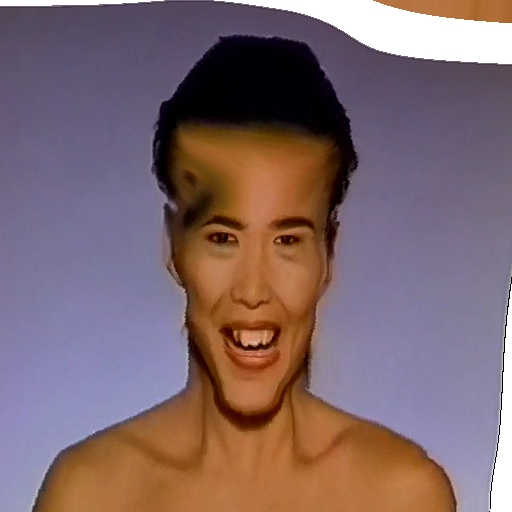
\includegraphics[width=\textwidth]{dst/dest0} % Replace 'image7' with your image file name
		\caption{}
	\end{subfigure}
	% ... (Add subfigures for the second row)
	
		    
	\caption{Ziel- zu Quell warps}
	\label{fig:destinations}
\end{figure}

Die Sequenz in Abbildung \ref{fig:destinations} muss zunaechst noch
in ihrer Reihenfolge geaendert werden bevor
die Kreuzblende angewendet wird.

\begin{figure}[htbp]
	\centering

		    	
	\begin{subfigure}[b]{0.4\textwidth}
		\centering
		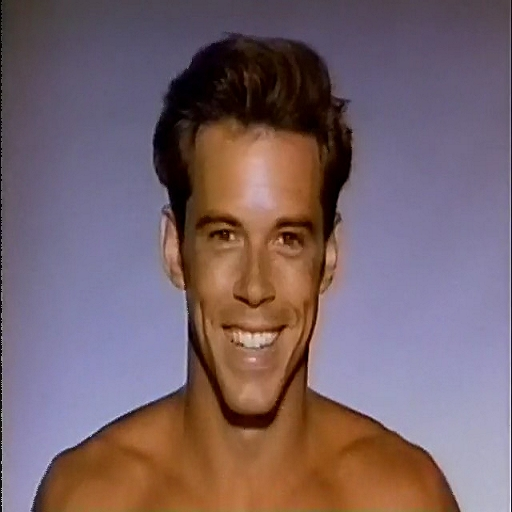
\includegraphics[width=\textwidth]{final/final0} % Replace 'image7' with your image file name
		\caption{}
	\end{subfigure}
	\begin{subfigure}[b]{0.4\textwidth}
		\centering
		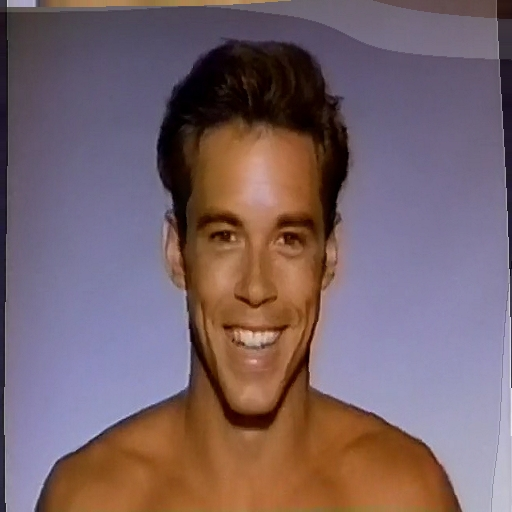
\includegraphics[width=\textwidth]{final/final1} % Replace 'image7' with your image file name
		\caption{}
	\end{subfigure}
	\begin{subfigure}[b]{0.4\textwidth}
		\centering
		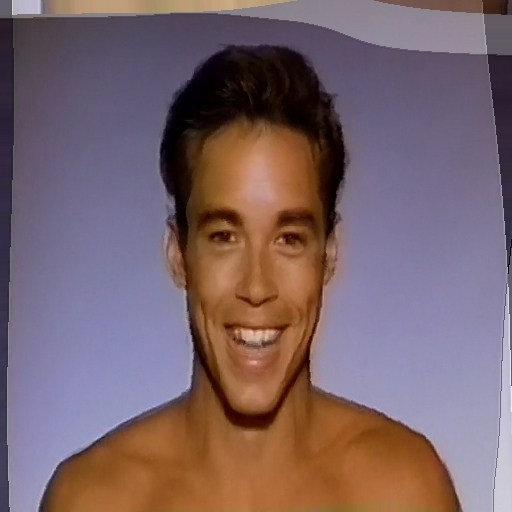
\includegraphics[width=\textwidth]{final/final2} % Replace 'image7' with your image file name
		\caption{}
	\end{subfigure}
	\begin{subfigure}[b]{0.4\textwidth}
		\centering
		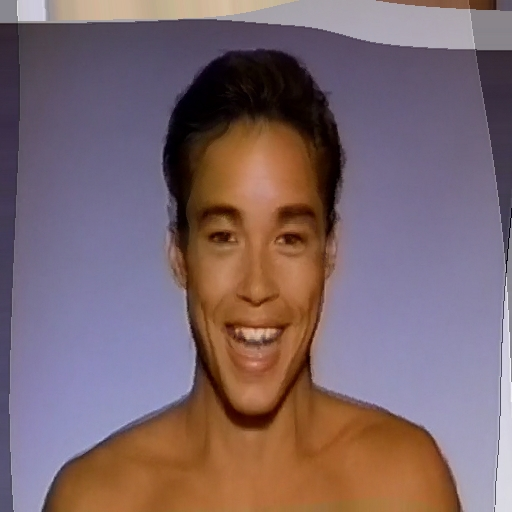
\includegraphics[width=\textwidth]{final/final3} % Replace 'image7' with your image file name
		\caption{}
	\end{subfigure}
	\begin{subfigure}[b]{0.4\textwidth}
		\centering
		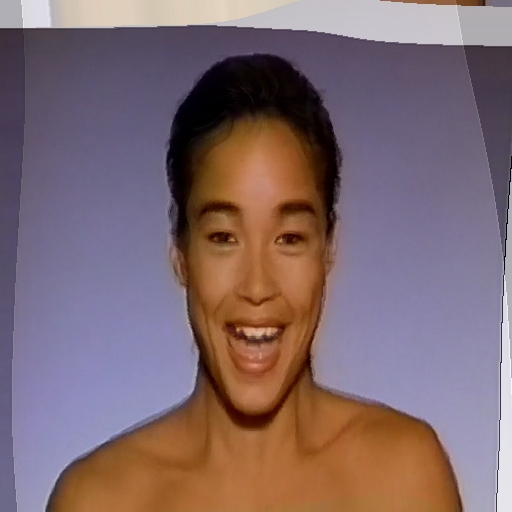
\includegraphics[width=\textwidth]{final/final4} % Replace 'image7' with your image file name
		\caption{}
	\end{subfigure}
	\begin{subfigure}[b]{0.4\textwidth}
		\centering
		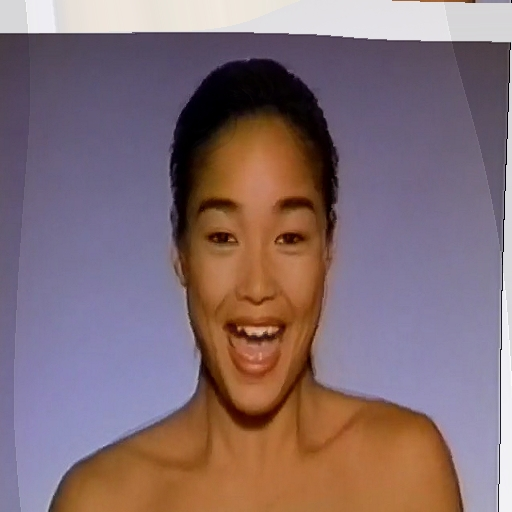
\includegraphics[width=\textwidth]{final/final5} % Replace 'image7' with your image file name
		\caption{}
	\end{subfigure}
	\begin{subfigure}[b]{0.4\textwidth}
		\centering
		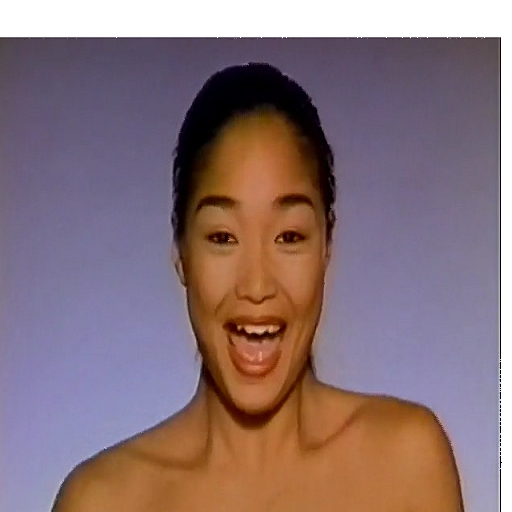
\includegraphics[width=\textwidth]{final/final6} % Replace 'image7' with your image file name
		\caption{}
	\end{subfigure}
	% ... (Add subfigures for the second row)
			    
	\caption{Finale Komposition}
	\label{fig:final}
\end{figure}



\appendix
\chapter{Software}

Fuer den Kurs haben wir eine Beispielanwendung, PowerMorph, erstellt.
Fuer das Bauen wird ein CMake file bereitgestellt. Die Software basiert
auf OpenGL 3.0 und ist somit auch auf MacOS lauffaehig (zwar hat Apple
den Support von OpenGL eingestellt, allerdings werden Anwendungen, welche bis
einschl. maximal Version 4.1 von OpenGL verwenden, nach wie vor unterstuetzt).
Ausserdem nutzen wir folgende externe Bibliotheken:

\begin{itemize}
	\item \textbf{SDL2} als Abstraktion zum Betriebssystem fuer Fenster und OpenGL context Erstellung.
	\href{https://github.com/libsdl-org/SDL}{https://github.com/libsdl-org/SDL} 
	\item \textbf{STB image/image write}: Lesen/Schreiben von Bilddateien.
		\href{https://github.com/nothings/stb}{https://github.com/nothings/stb} 
	\item \textbf{GLM}: Mathematik Bibliothek, die gut mit OpenGL zusammenarbeitet. 
			\href{https://github.com/g-truc/glm}{https://github.com/g-truc/glm}
	\item \textbf{Dear ImGUI}: Immediate Mode GUI Bibliothek fuer den Editor.
	\item \textbf{tinyfiledialogs}: Betriebssystemunabhaengige Bibliothek fuer Window-Messages, Oeffnen/Speichern Dialoge.
	\item \textbf{GIF writer by Charlie Tangora}: Speichern der gerenderten Sequenzen als GIF.
				\href{https://github.com/charlietangora/gif-h}{https://github.com/charlietangora/gif-h} 
\end{itemize}

\section{Installation}

Wir nutzen CMake, um Projektdateien
fuer eine IDE bzw. Makefiles zu generieren. 

Nach der Installation ist sollte die Software ohne weiteres Aufrufbar sein. Ein fertiges Binary fuer Windows 64 bit ist auf 
www.nocheinfuegen.de herunterladbar.

\section{Verwenden von PowerMorph}

Die Bedienung ist weitestgehend selbsterklaerend. Im Source
Fenster wird eine Linie fuer ein Feature gezogen. Per
Mausklick wird der Fusspunkt der Linie gesetzt, ein weiterer
Mausklick vervollstaendigt diese. Dabei ist die Richtung der Linie
durch den letzten Klick gegeben. Danach muss
im Destination Fenster eine weitere Linie erzeugt werden, um das
Paar zu komplettieren. Dieses Vorgehen kann so lange wiederholt
werden, wie gewuenscht. Eine bereits gesetzte Linie kann immer mit
der Tastenkombination CTRL+Z rueckgaengig gemacht werden.
Ist man mit der Definition der Features zufrieden, koennen mit einem
Klick auf den \textbf{MAGIC!}-Button die Morphs von Quell- und Zielbild
generiert und danach ueberblendet werden. Je nach Aufloesung des Bilderpaares
und der Anzahl der gesetzen Linien kann dieser Vorgang ein wenig
dauern. Ist die Berechnung abgeschlossen, so wird ein
neues \textbf{Result}-Fenster geoeffnet. Dort laesst sich das
Resultat begutachten.

\section{Ausblick}




%\chapter{Figures}

\vspace*{-3in}

\begin{figure}
\vspace{2.4in}
\caption{Armadillo slaying lawyer.}
\label{arm:fig1}
\end{figure}
\clearpage
\newpage

\begin{figure}
\vspace{2.4in}
\caption{Armadillo eradicating national debt.}
\label{arm:fig2}
\end{figure}
\clearpage
\newpage

%% This defines the bibliography file (main.bib) and the bibliography style.
%% If you want to create a bibliography file by hand, change the contents of
%% this file to a `thebibliography' environment.  For more information 
%% see section 4.3 of the LaTeX manual.
%\begin{singlespace}
\bibliography{main}
\bibliographystyle{plain}
%\end{singlespace}

\end{document}

